
%\subsection{Coordonnées}
\SbSSCT{Coordonnées}{Coordinates}
\begin{center}
\RRR{13-2-1}
\end{center}

%\subsubsection{Système de coordonnées \og canvas \fg}
\SbSbSSCT{Système de coordonnées \og canvas \fg}{Canvas coordinates}

\tikzset{every picture/.style=blue,very thick,inner sep=0pt}

\begin{tabular}{|c|c|} \hline 
\TFRGB{Explicite}{explicit}  & \TFRGB{Implicite}{implicit}
\\ \hline
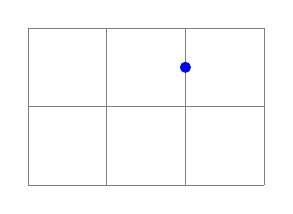
\begin{tikzpicture}
\draw[help lines] (0,0) grid (3,2);
\fill (canvas cs:x=2cm,y=1.5cm) circle (2pt);
\end{tikzpicture}
&
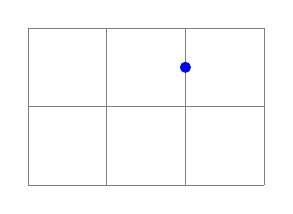
\begin{tikzpicture}
\draw[help lines] (0,0) grid (3,2);
\fill (2,1.5) circle (2pt);
\end{tikzpicture}

\\ \hline  
 \BS{fill} (\RDD{canvas cs}:x=2cm,y=1.5cm) circle (2pt);
& \BS{fill} {\color{blue}(2cm,1.5cm)} circle (2pt);
\\ \hline 
\end{tabular} 


%\subsubsection{Système de coordonnées  xyz}
\SbSbSSCT{Système de coordonnées  xyz}{xyz coordinates}

\begin{tabular}{|c|c|c|} \hline 
\begin{tikzpicture}[->]
\draw (0,0) -- (xyz cs:x=1);
\draw (0,0) -- (xyz cs:y=1);
\draw (0,0) -- (xyz cs:z=1);
\end{tikzpicture}
&
\begin{tikzpicture}[->]
\draw (0,0) -- (1,0,0);
\draw (0,0) -- (0,1,0);
\draw (0,0) -- (0,0,1);
\end{tikzpicture}
\\ \hline 
\BS{draw} (0,0) - - (\RDD{xyz cs}:x=1); & \BS{draw}  (0,0) - - (1,0,0); \\
\BS{draw}  (0,0) - - (\RDD{xyz cs}:y=1); &  \BS{draw} (0,0) - - (0,1,0); \\
\BS{draw} (0,0) - - (\RDD{xyz cs}:z=1); &  \BS{draw}  (0,0) - - (0,0,1); 
\\ \hline 

\end{tabular} 

%\subsubsection{Système de coordonnées polaire \og canvas \fg}
\SbSbSSCT{Système de coordonnées polaire \og canvas \fg}{Polar coordinates}

\begin{tabular}{|c|c|c|} \hline
\TFRGB{Explicite}{explicit}  & \TFRGB{Implicite}{implicit}
\\ \hline
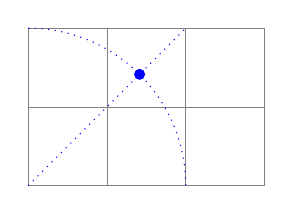
\begin{tikzpicture}
\draw[help lines] (0,0) grid (3,2);
\draw [dotted](0,2) arc (90 :0 :2);
\draw [dotted](0,0) --(2,2);
\fill (canvas polar cs:angle=45,radius=2cm) circle (2pt);
\end{tikzpicture}
&
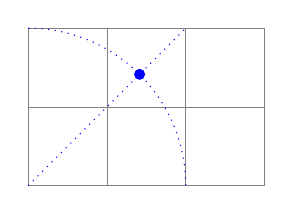
\begin{tikzpicture}
\draw[help lines] (0,0) grid (3,2);
\draw [dotted](0,2) arc (90 :0 :2);
\draw [dotted](0,0) --(2,2);
\fill (45:2cm) circle (2pt);
\end{tikzpicture}
\\ \hline 
\BS{fill} (\RDD{canvas polar cs}:\RDD{angle}=45,\RDD{radius}=2cm) circle (2pt);
&
\BS{fill} {\color{blue}(45:2cm)} circle (2pt);
\\ \hline 
\end{tabular} 

\bigskip
\begin{tabular}{|c|} \hline  
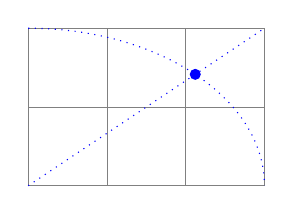
\begin{tikzpicture}
\draw[help lines] (0,0) grid (3,2);
\draw [dotted](0,2) arc (90 :0 :3 and 2);
\draw [dotted](0,0) --(3,2);
\fill (canvas polar cs:angle=45,x radius=3cm,y radius=2cm) circle (2pt);
\end{tikzpicture}
\\ \hline  
\BS{fill} (canvas polar cs:angle=45,\RDD{x radius}=3cm,\RDD{y radius}=2cm) circle (2pt);
\\ \hline 
\end{tabular} 



\newpage
%\subsubsection{Coordinate system xyz polar} % A VOIR
\SbSbSSCT{Coordinate system xyz polar}{Coordinate system xyz polar}

\begin{tabular}{|c|c|c|} \hline
\TFRGB{Explicite}{explicit}  & \TFRGB{Implicite}{implicit}
\\ \hline
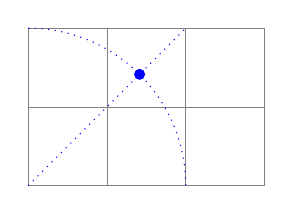
\begin{tikzpicture}
\draw[help lines] (0,0) grid (3,2);
\draw [dotted](0,2) arc (90 :0 :2);
\draw [dotted](0,0) --(2,2);
\fill (xyz polar cs:angle=45,radius=2) circle (2pt);
\end{tikzpicture}
&
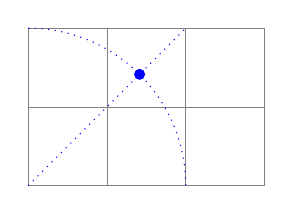
\begin{tikzpicture}
\draw[help lines] (0,0) grid (3,2);
\draw [dotted](0,2) arc (90 :0 :2);
\draw [dotted](0,0) --(2,2);
\fill (45:2) circle (2pt);
\end{tikzpicture}
\\ \hline 
\BS{fill} (\RDD{xyz polar cs}:\RDD{angle}=45,\RDD{radius}=2) circle (2pt);
&
\BS{fill} {\color{blue}(45:2cm)} circle (2pt);
\\ \hline 
\end{tabular} 

\bigskip
\begin{tabular}{|c|} \hline  
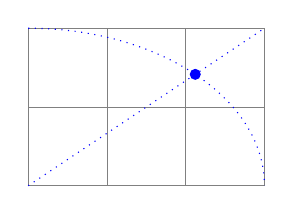
\begin{tikzpicture}
\draw[help lines] (0,0) grid (3,2);
\draw [dotted](0,2) arc (90 :0 :3 and 2);
\draw [dotted](0,0) --(3,2);
\fill (xyz polar cs:angle=45,x radius=3,y radius=2) circle (2pt);
\end{tikzpicture}
\\ \hline  
\BS{fill} (xyz polar cs:angle=45,\RDD{x radius}=3,\RDD{y radius}=2) circle (2pt);
\\ \hline 
\end{tabular} 

\bigskip

\begin{tabular}{|c|c|c|} \hline
\multicolumn{2}{|c|}{\BS{begin}\AC{tikzpicture}{\color{red}[x=1.5cm,y=1cm]} }
\\ \hline
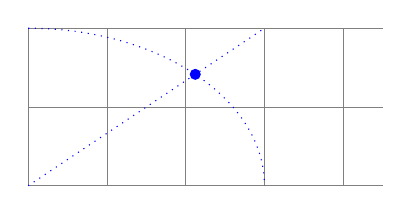
\begin{tikzpicture}[x=1.5cm,y=1cm]
\draw[help lines] (0,0) grid (3,2);
\draw [dotted](0,2) arc (90 :0 :2);
\draw [dotted](0,0) --(2,2);
\fill (xyz polar cs:angle=45,radius=2) circle (2pt);
\end{tikzpicture}
&
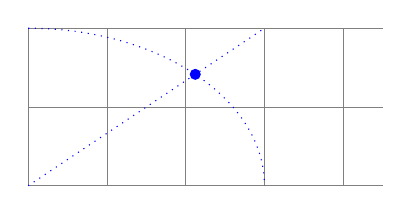
\begin{tikzpicture}[x=1.5cm,y=1cm]
\draw[help lines] (0,0) grid (3,2);
\draw [dotted](0,2) arc (90 :0 :2);
\draw [dotted](0,0) --(2,2);
\fill (45:2) circle (2pt);
\end{tikzpicture}
\\ \hline 
\BS{fill} (\RDD{xyz polar cs}:\RDD{angle}=45,\RDD{radius}=2) circle (2pt);
&
\BS{fill} {\color{blue}(45:2cm)} circle (2pt);
\\ \hline 
\end{tabular} 
\bigskip

\begin{tabular}{|c|c|c|} \hline
\multicolumn{2}{|c|}{\BS{begin}\AC{tikzpicture}{\color{red}[x=\AC{(0cm,1cm)},y=\AC{(-1cm,0cm)}]} }
\\ \hline
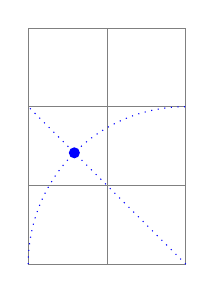
\begin{tikzpicture}[x={(0cm,1cm)},y={(-1cm,0cm)}]
\draw[help lines] (0,0) grid (3,2);
\draw [dotted](0,2) arc (90 :0 :2);
\draw [dotted](0,0) --(2,2);
\fill (xyz polar cs:angle=45,radius=2) circle (2pt);
\end{tikzpicture}
&
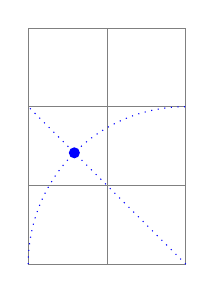
\begin{tikzpicture}[x={(0cm,1cm)},y={(-1cm,0cm)}]
\draw[help lines] (0,0) grid (3,2);
\draw [dotted](0,2) arc (90 :0 :2);
\draw [dotted](0,0) --(2,2);
\fill (45:2) circle (2pt);
\end{tikzpicture}
\\ \hline 
\BS{fill} (\RDD{xyz polar cs}:\RDD{angle}=45,\RDD{radius}=2) circle (2pt);
&
\BS{fill} {\color{blue}(45:2cm)} circle (2pt);
\\ \hline 
\end{tabular} 



%--------------------------------------------------------
%\subsubsection{Coordonnées barycentriques}
\SbSbSSCT{Coordonnées barycentriques}{Barycentric coordinates}

\begin{center}
\RRR{13-2-2}
\end{center}

\begin{tabular}{|c|c|c|} \hline
\multicolumn{3}{|c|}{  \BS{node} [circle,fill=red!20] at (\RDD{barycentric cs}:A=0.6,B=0.3 ) \AC{X};   }\\ 
\hline
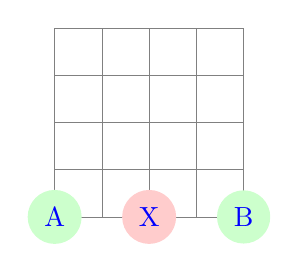
\begin{tikzpicture}[scale=.6]
\draw[help lines] (0,0) grid (4,4);
\node[circle,fill=green!20,] (A) at (0,0) {A};
\node[circle,fill=green!20,] (B) at (4,0) {B};
\node[circle,fill=red!20] at (barycentric cs:A=0.3,B=0.3 ) {X};
\end{tikzpicture}
&
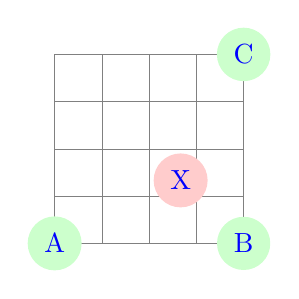
\begin{tikzpicture}[scale=.6]
\draw[help lines] (0,0) grid (4,4);
\node[circle,fill=green!20,] (A) at (0,0) {A};
\node[circle,fill=green!20,] (B) at (4,0) {B};
\node[circle,fill=green!20,] (C) at (4,4) {C};
\node[circle,fill=red!20] at (barycentric cs:A=0.4,B=0.4 ,C=.4) {X};
\end{tikzpicture}
&
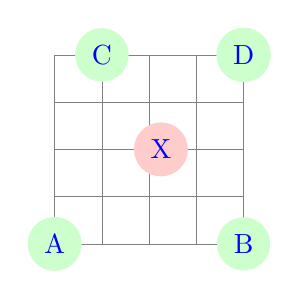
\begin{tikzpicture}[scale=.6]
\draw[help lines] (0,0) grid (4,4);
\node[circle,fill=green!20,] (A) at (0,0) {A};
\node[circle,fill=green!20,] (B) at (4,0) {B};
\node[circle,fill=green!20,] (C) at (1,4) {C};
\node[circle,fill=green!20,] (D) at (4,4) {D};
\node[circle,fill=red!20] at (barycentric cs:A=0.5,B=0.5,C=.5,D=.5 ) {X};
\end{tikzpicture}
\\ \hline
A=0.3,B=0.3 & A=0.4,B=0.4 ,C=.4 & A=0.5,B=0.5,C=.5,D=.5 
\\ \hline
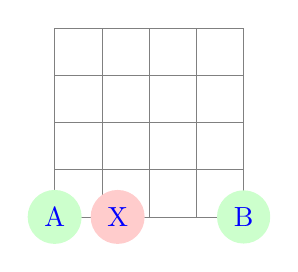
\begin{tikzpicture}[scale=.6]
\draw[help lines] (0,0) grid (4,4);
\node[circle,fill=green!20,] (A) at (0,0) {A};
\node[circle,fill=green!20,] (B) at (4,0) {B};
\node[circle,fill=red!20] at (barycentric cs:A=0.6,B=0.3 ) {X};
\end{tikzpicture}
&
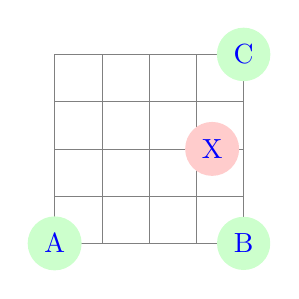
\begin{tikzpicture}[scale=.6]
\draw[help lines] (0,0) grid (4,4);
\node[circle,fill=green!20,] (A) at (0,0) {A};
\node[circle,fill=green!20,] (B) at (4,0) {B};
\node[circle,fill=green!20,] (C) at (4,4) {C};
\node[circle,fill=red!20] at (barycentric cs:A=0.2,B=0.4 ,C=.6) {X};
\end{tikzpicture}
&
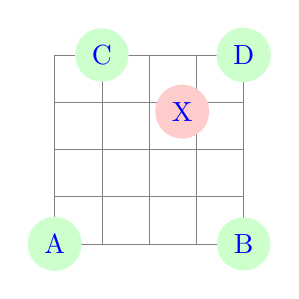
\begin{tikzpicture}[scale=.6]
\draw[help lines] (0,0) grid (4,4);
\node[circle,fill=green!20,] (A) at (0,0) {A};
\node[circle,fill=green!20,] (B) at (4,0) {B};
\node[circle,fill=green!20,] (C) at (1,4) {C};
\node[circle,fill=green!20,] (D) at (4,4) {D};
\node[circle,fill=red!20] at (barycentric cs:A=0.2,B=0.4,C=.6,D=.8 ) {X};
\end{tikzpicture}
\\ \hline
A=0.6,B=0.3 & A=0.2,B=0.4 ,C=.6 & A=0.2,B=0.4,C=.6,D=.8
\\ \hline
\end{tabular}


%\subsection{Coordonnées nominatives : n\oe ud}
\SbSbSSCT{Coordonnées nominatives : n\oe ud}{Named coordinates: nodes}

\begin{center}
\RRR{13-2-3}
\end{center}

\begin{tabular}{|c|c|} \hline  
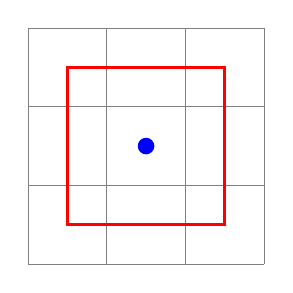
\begin{tikzpicture}[blue,very thick,baseline=1cm]
\draw[help lines] (0,0) grid (3,3);
\coordinate (centre) at (1.5,1.5) ;
\coordinate (A) at (.5,.5) ;
\coordinate (B) at (2.5,2.5) ;
\fill (centre) circle (3pt);
\draw[red] (A) rectangle (B) ;
\end{tikzpicture}
&  
\parbox[c]{8cm}{
\BSS{coordinate} {\color{blue}(centre)} at(1.5,1.5) ; \\
\BSS{coordinate} {\color{blue}(A)} at (.5,.5) ;\\
\BSS{coordinate} {\color{blue}(B)} at  (2.5,2.5) ;\\
\\
\BS{fill} {\color{blue}(centre)} circle (3pt);\\
\BS{draw}[red] {\color{blue}(A)} rectangle {\color{blue}(B)} ;\\
}
\\ \hline 
\end{tabular} 

\TFRGB{voir aussi}{see also} page \pageref{nomnoeud}

%---------------------------------------------------------
%\subsubsection{Coordonnées relatives à un noeud}
\SbSbSSCT{Coordonnées relatives à un noeud}{Coordinates relative to a node}

\begin{tabular}{|c|c|c|c|} \hline
\multicolumn{4}{|l|}{  \BS{node} [draw,fill=green!20,] (A) at (1,1) \AC{\BS{huge}  noeud}; }\\ 
\multicolumn{4}{|l|}{  \BS{fill}[red] (\RDD{node cs}:\RDD{name}=A,\RDD{anchor}=south) circle (3pt);   }\\ 
\hline

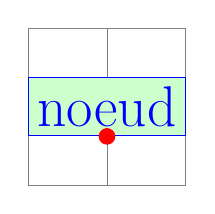
\begin{tikzpicture}
\draw[help lines] (0,0) grid (2,2);
\node[draw,fill=green!20,] (A) at (1,1) {\huge noeud};
\fill[red] (node cs:name=A,anchor=south) circle (3pt);
\end{tikzpicture}
&
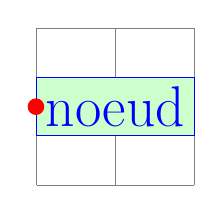
\begin{tikzpicture}
\draw[help lines] (0,0) grid (2,2);
\node[draw,fill=green!20,] (A) at (1,1) {\huge noeud};
\fill[red] (node cs:name=A,anchor=west) circle (3pt);
\end{tikzpicture}
&
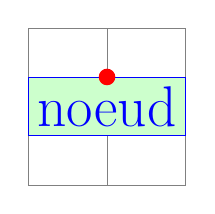
\begin{tikzpicture}
\draw[help lines] (0,0) grid (2,2);
\node[draw,fill=green!20,] (A) at (1,1) {\huge noeud};
\fill[red] (node cs:name=A,anchor=north) circle (3pt);
\end{tikzpicture}
&
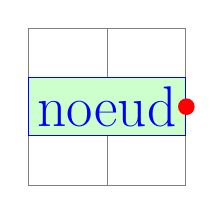
\begin{tikzpicture}
\draw[help lines] (0,0) grid (2,2);
\node[draw,fill=green!20,] (A) at (1,1) {\huge noeud};
\fill[red] (node cs:name=A,anchor=east) circle (3pt);
\end{tikzpicture}
\\ \hline
name=A,anchor=south & name=A,anchor=west & name=A,anchor=north & name=A,anchor=east
\\ \hline
\end{tabular}

\bigskip
\begin{tabular}{|c|c|c|c|} \hline
\multicolumn{4}{|c|}{  \BS{fill}[red] (node cs:\RDD{name}=A,\RDD{angle}=0) circle (3pt);  }\\ 
\hline

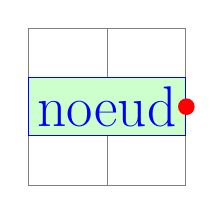
\begin{tikzpicture}
\draw[help lines] (0,0) grid (2,2);
\node[draw,fill=green!20,] (A) at (1,1) {\huge noeud};
\fill[red] (node cs:name=A,angle=0) circle (3pt);
\end{tikzpicture}
&
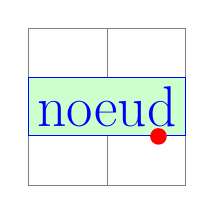
\begin{tikzpicture}
\draw[help lines] (0,0) grid (2,2);
\node[draw,fill=green!20,] (A) at (1,1) {\huge noeud};
\fill[red] (node cs:name=A,angle=-30) circle (3pt);
\end{tikzpicture}
&
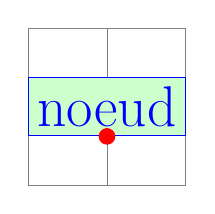
\begin{tikzpicture}
\draw[help lines] (0,0) grid (2,2);
\node[draw,fill=green!20,] (A) at (1,1) {\huge noeud};
\fill[red] (node cs:name=A,angle=-90) circle (3pt);
\end{tikzpicture}
&
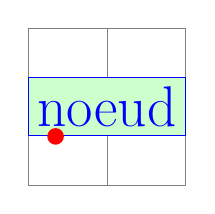
\begin{tikzpicture}
\draw[help lines] (0,0) grid (2,2);
\node[draw,fill=green!20,] (A) at (1,1) {\huge noeud};
\fill[red] (node cs:name=A,angle=-150) circle (3pt);
\end{tikzpicture}
\\ \hline
name=A,angle=0 & name=A,angle=-30 & nname=A,angle=-90 & name=A,angle=-150
\\ \hline
\end{tabular}


% % % % % % % % % % % % % % % % A voir % % % % % % % % % % % % % % % % %


%\subsubsection{Coordonnée à un intersection}
%
%\begin{tikzpicture}
%\draw[help lines] (0,0) grid (3,3);
%%\draw (intersection cs: first line={(A)- -(B)},second line={(1,2)- -(3,0)})coordinate (C);
%%\fill[red](C) circle (2pt);
%%\draw (C) circle (1cm);
%%\node [above]at(C){C};
%\end{tikzpicture}

%\subsubsection{ Coordonnée relative à 2 points}
\SbSbSSCT{Coordonnées relatives à deux points}{Coordinates relative to two points}
\begin{center}
\RRR{13-3-1}
\end{center}

\begin{tabular}{|c|c|} \hline
\multicolumn{2}{|c|}{  \BS{node} [circle,fill=red!20] at (1,1 {\color{red}|-} 3,3) \AC{X}   }\\ 
\hline
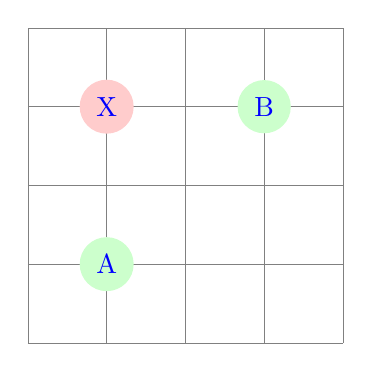
\begin{tikzpicture}
\draw[help lines] (0,0) grid (4,4);
\node[circle,fill=green!20,] (A) at (1,1) {A};
\node[circle,fill=green!20,] (B) at (3,3) {B};
\node[circle,fill=red!20] at (1,1 |- 3,3) {X};
\end{tikzpicture}
&
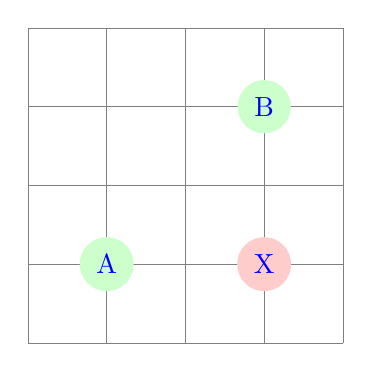
\begin{tikzpicture}
\draw[help lines] (0,0) grid (4,4);
\node[circle,fill=green!20,] (A) at (1,1) {A};
\node[circle,fill=green!20,] (B) at (3,3) {B};
\node[circle,fill=red!20] at (1,1 -| 3,3) {X};
\end{tikzpicture}
\\ \hline
at (1,1 {\color{red}|-} 3,3)
&
at (1,1 {\color{red}-|} 3,3)
\\ \hline
\end{tabular}


\newpage
%\subsubsection{ Coordonnée relative à une intersection}
\SbSbSSCT{Coordonnée relative à une intersection}{Coordinates relative to an intersection}
\begin{center}
\RRR{13-3-2}
\end{center}

 \maboite{\BS{usetikzlibrary}\AC{intersections}}
\label{lib-intersections}


\begin{tabular}{|c|c|c|c|} \hline 
\multicolumn{4}{|l|}{  \BS{draw} [\RDD{name path}=cercle] (2,1) circle  (1cm);   }\\ 
\multicolumn{4}{|l|}{  \BS{draw} [\RDD{name path}=rectangle] (0.5,0.5) rectangle +(3,1);   }\\ 
\multicolumn{4}{|l|}{ \BS{fill} [red,\RDD{ name intersections}=\AC{of=cercle and rectangle}]
(\RDD{intersection}-1) circle (2pt)   }\\ 
\hline 
\begin{tikzpicture}[scale=.8]
\draw [help lines] grid (4,2);
\draw [name path=cercle] (2,1) circle  (1cm);
\draw [name path=rectangle] (0.5,0.5) rectangle +(3,1);
\fill [red, name intersections={of=cercle and rectangle}]
(intersection-1) circle (2pt)  ;
\end{tikzpicture}
& 
\begin{tikzpicture}[scale=.8]
\draw [help lines] grid (4,2);
\draw [name path=cercle] (2,1) circle  (1cm);
\draw [name path=rectangle] (0.5,0.5) rectangle +(3,1);
\fill [red, name intersections={of=cercle and rectangle}] (intersection-2) circle (2pt) ;
\end{tikzpicture} 
&  
\begin{tikzpicture}[scale=.8]
\draw [help lines] grid (4,2);
\draw [name path=cercle] (2,1) circle  (1cm);
\draw [name path=rectangle] (0.5,0.5) rectangle +(3,1);
\fill [red, name intersections={of=cercle and rectangle}] (intersection-3) circle (2pt) ;
\end{tikzpicture}
&  
\begin{tikzpicture}[scale=.8]
\draw [help lines] grid (4,2);
\draw [name path=cercle] (2,1) circle  (1cm);
\draw [name path=rectangle] (0.5,0.5) rectangle +(3,1);
\fill [red, name intersections={of=cercle and rectangle}] (intersection-4) circle (2pt) ;
\end{tikzpicture}
\\ 
\hline intersection-1 & intersection-2 &intersection-3  & intersection-4 \\ 
\hline 
\end{tabular} 

\bigskip

\begin{tabular}{|c|} \hline  
\BS{fill} [red, name intersections=\AC{of=cercle and rectangle}] \\
(intersection-1) circle (2pt) {\color{red} node[black,above right] \AC{point a}} ;
\\ \hline  
\begin{tikzpicture}
\draw [help lines] grid (4,2);
\draw [name path=cercle] (2,1) circle  (1cm);
\draw [name path=rectangle] (0.5,0.5) rectangle +(3,1);
\fill [red, name intersections={of=cercle and rectangle}]
(intersection-1) circle (2pt) node[black,above right] {point a} ;
\end{tikzpicture} 
\\ \hline 
\end{tabular} 




\bigskip

\begin{tabular}{|c|} \hline 
\BS{fill} [red, name intersections=\AC{of=cercle and rectangle, \RDD{name}=point}]; \\
\BS{draw} [red] (point-1) - - (point-3); \BS{draw} [green] (point-2) - - (point-4);
\\ \hline  
\begin{tikzpicture}
\draw [help lines] grid (4,2);
\draw [name path=cercle] (2,1) circle  (1cm);
\draw [name path=rectangle] (0.5,0.5) rectangle +(3,1);
\fill [red, name intersections={of=cercle and rectangle, name=point}];
\draw [red] (point-1) -- (point-3);
\draw [green] (point-2) -- (point-4);
\end{tikzpicture}
\\ \hline 
\end{tabular} 

\bigskip
\begin{tabular}{|c|} \hline  
\BS{fill} [red, name intersections=\AC{of=cercle and rectangle, \RDD{by}=\AC{a,b,c,d}}]; \\
\BS{draw} [red] (a) - - (c); \hspace{1cm} \BS{draw} [green] (b) - - (d);
\\ \hline   
\begin{tikzpicture}
\draw [help lines] grid (4,2);
\draw [name path=cercle] (2,1) circle  (1cm);
\draw [name path=rectangle] (0.5,0.5) rectangle +(3,1);
\fill [red, name intersections={of=cercle and rectangle, by={a,b,c,d}}];
\draw [red] (a) -- (c);
\draw [green] (b) -- (d);
\end{tikzpicture}
\\ \hline 
\end{tabular} 

\bigskip

\begin{tabular}{|c|} \hline  
\BS{fill} [name intersections=\AC{of=cercle and rectangle, name=i, \RDD{total}=\BS{t}}] [red] \\
\BS{foreach} \BS{s} in \AC{1,...,\BS{t}} \AC{(i-\BS{s}) circle (2pt) node[black,above right] \AC{\BS{s}}}
\\ \hline  
\begin{tikzpicture}
\draw [help lines] grid (4,2);
\draw [name path=cercle] (2,1) circle  (1cm);
\draw [name path=rectangle] (0.5,0.5) rectangle +(3,1);
\fill [name intersections={of=cercle and rectangle, name=i, total=\t}]
[red]
\foreach \s in {1,...,\t}{(i-\s) circle (2pt) node[black,above right] {\s}};
\end{tikzpicture}
\\ \hline 
\end{tabular} 



%\begin{tikzpicture}
%\clip (-0.5,-0.75) rectangle (3.25,2.25);
%\foreach \pathname/\shift in {line/0cm, curve/2cm}{
%\tikzset{xshift=\shift}
%\draw [->, name path=curve] (1,1.5) .. controls (-1,1) and (2,0.5) .. (0,0);
%
%\draw [->, name path=line] (0,-.5) -- (1,2) ;
%
%\fill [name intersections={of=line and curve,sort by=\pathname, name=i}]
%[red, opacity=0.5, every node/.style={left=.25cm, black, opacity=1}]
%\foreach \s in {1,2,3}{(i-\s) circle (2pt) node {\footnotesize\s}};
%}
%\end{tikzpicture}
%---------------------------------------------------------------------------
\newpage

%\subsection{Position calculée}
\SbSSCT{Position calculée}{Calculated positions}

%\subsubsection{Position calculée avec le module  \og  pgfmath \fg}
\SbSbSSCT{Position calculée avec le module  \og  pgfmath \fg}{Calculated positions with  \og  pgfmath \fg }

\begin{center}
\RRR{13-2-1}
\end{center}

\TFRGB{Ce module est chargé automatiquement avec le module Tikz}{Package automatically loaded with Tikz} 

\begin{tabular}{|c|} \hline 
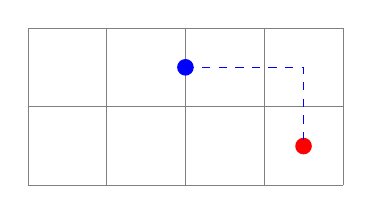
\begin{tikzpicture}
\draw[help lines] (0,0) grid (4,2);
\fill [red] (canvas cs:x=2cm+1.5cm,y=1.5cm-1cm) circle (3pt);
\fill [blue] (2cm,1.5cm) circle (3pt);
\draw[dashed] (2,1.5) -| (3.5,.5);
\end{tikzpicture}
\\ \hline  
\emph{Explicite} : \BS{fill} [red] (\RDD{canvas cs}:x=2cm+1.5cm,y=1.5cm-1cm) circle (3pt);
 \\  \hline 
\emph{Implicite} :  \BS{fill} [red] {\color{red}(2cm+1.5cm,1.5cm-1cm)} circle (3pt);
\\ \hline 
\end{tabular} 

\bigskip
\begin{tabular}{|c|c|c|} \hline 
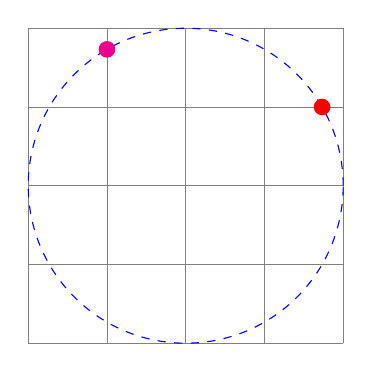
\begin{tikzpicture}[baseline=0pt]
\draw[help lines] (0,0) grid (4,4);
 \draw[dashed] (2,2) circle (2);
\fill[red](2+ 2*cos 30,2+2*sin 30) circle (3pt);
\fill[magenta](2+ 2*cos{(120)},2+2*sin{(120)}) circle (3pt);
\end{tikzpicture}
&
\parbox[c]{8cm}{
 \BS{draw}[dashed] (2,2) circle (2);\\
 \smallskip
 \BS{fill} [red]{\color{red}(2+ 2*cos 30 , 2+2*sin 30)} circle (3pt);\\
  \smallskip
 \BS{fill}[magenta] {\color{red}(2+2*cos\AC{(120)} , 2+2*sin\AC{(120)})} circle (3pt); 
 }
\\ \hline 
\end{tabular} 
%
%\subsubsection{Position calculée avec \og librairy calc \fg}
\SbSSCT{Position calculée avec \og librairy calc \fg}{Calculated positions with \og  calc  librairy calc \fg}

\begin{center}
\RRR{13-5}
\end{center}
\label{lib-calc}
%Insérer dans le préambule : 

 \maboite{\BS{usetikzlibrary}\AC{calc}}
 
\begin{tabular}{|c|c|} \hline  
\begin{tikzpicture}[baseline=0pt]
\draw [help lines] (0,0) grid (3,2);
\node (a) at (1,1) {A};
\fill [red] ($(a) + 2/3*(1cm,0)$) circle (2pt);
\fill [red] ($(a) + 4/3*(1cm,0)$) circle (2pt);
\end{tikzpicture}
&
\parbox{8cm}{
\BS{node} (a) at (1,1) \AC{A}; \\
\BS{fill} [red] {\color{red} (\$(a) + 2/3*(1cm,0)\$)} circle (2pt); \\
\BS{fill} [red] {\color{red}(\$(a) + 4/3*(1cm,0)\$)} circle (2pt); \\
}
\\ 
\hline 
\end{tabular} 


%\subsubsection{Tangentes avec \og librairy calc \fg}
\SbSSCT{Tangentes avec \og librairy calc \fg}{Tangents with  \og calc librairy  \fg}

\begin{center}
\RRR{13-2-4}
\end{center}

\begin{tabular}{|c|c|} \hline 
\multicolumn{2}{|l|}{\BS{node}[fill=green!20] (a) at (3,1.5) \AC{A}; } \\
\multicolumn{2}{|l|}{\BS{fill}[red] (\RDD{tangent cs}:\RDD{node}=c,\RDD{point}=\AC{(A)},\RDD{solution}=1);  }\\ 
%\multicolumn{2}{|l|}{\BS{draw}[red] (1,1) - -(\RDD{tangent} cs:\RDD{node}=c,\RDD{point}=\AC{(3,1.5)} ,\RDD{solution}=1); }\\ 
\hline
\begin{tikzpicture}
\draw[help lines] (0,0) grid (4,2);
\node[fill=green!20] (A) at (3,1.5) {A};
\node [circle,draw] (c) at (1,1) [minimum size=1.5cm] {$c$};
\draw[red,dashed] (A) - -(tangent cs:node=c,point={(A)},solution=1) ;
\draw[red,dashed] (1,1) - -(tangent cs:node=c,point={(3,1.5)},solution=1) ;
\fill[red] (tangent cs:node=c,point={(A)},solution=1) circle (3pt);
\end{tikzpicture}
&
\begin{tikzpicture}
\draw[help lines] (0,0) grid (4,2);
\node[fill=green!20] (A) at (3,1.5) {A};
\node [circle,draw] (c) at (1,1) [minimum size=1.5cm] {$c$};
\draw[red,dashed] (A) - -(tangent cs:node=c,point={(A)},solution=2) ;
\draw[red,dashed] (1,1) - -(tangent cs:node=c,point={(A)},solution=2) ;
\fill[red] (tangent cs:node=c,point={(A)},solution=2) circle (3pt);
\end{tikzpicture}
\\ \hline
\RDD{solution}=1 & \RDD{solution}=2
\\ \hline
\end{tabular} 

\newpage

%\subsubsection{Point à pourcentage donné }
\SbSbSSCT{Point à pourcentage donné }{Percentage position }

\begin{center}
\RRR{13-5-3}
\end{center}


\begin{tabular}{|c|c|} \hline  
\multicolumn{2}{|c|}{\BS{fill}[red] ({\color{red}\$(0,1)!.25!(4,1)\$}) circle (4pt); } \\  \hline  

\begin{tikzpicture}
\draw [help lines] (0,0) grid (4,2);
\draw [line width= 3pt] (0,1) -- (4,1);
\fill[red] ($(0,1)!.25!(4,1)$) circle (4pt);
\end{tikzpicture}
&  
\begin{tikzpicture}
\draw [help lines] (0,0) grid (4,2);
\draw [line width= 3pt] (0,1) -- (4,1);
\fill[red] ($(0,1)!.75!(4,1)$) circle (4pt);
\end{tikzpicture}
\\ \hline (0,1)!{\color{red}0.25}!(4,1) & (0,1)!{\color{red}0.75}!(4,1) \\ 
\hline 
\end{tabular} 

\bigskip

\begin{tabular}{|c|} \hline  
\begin{tikzpicture}
\draw [help lines] (0,0) grid (4,3);
\draw [line width=2pt ](0,2) -- (4,2);
\draw[red] ($(0,2)!.75!(4,2)$) -- (0,0);
\fill[red] ($(0,2)!.75!(4,2)!.66!(0,0)$) circle (4pt);
\end{tikzpicture}
\\ \hline 
\BS{fill}[red] (\${\color{blue}(0,2)!0.75!(4,2)}!{\color{red}0.66!(0,0)}\$) circle (2pt);
\\ \hline 
\end{tabular} 



%\subsubsection{Point à distance donnée}
\SbSbSSCT{Point à distance donnée}{Position at a given distance }

\begin{center}
\RRR{13-5-4}
\end{center}

\begin{tabular}{|c|c|} \hline  
\multicolumn{2}{|c|}{\BS{fill}[red] ({\color{red}\$(0,1)!1.5cm!(4,1)\$}) circle (4pt); } \\  \hline  

\begin{tikzpicture}
\draw [help lines] (0,0) grid (4,2);
\draw [line width= 2pt] (0,1) -- (4,1);
\fill[red] ($(0,1)!1.5cm!(4,1)$) circle (4pt);
\end{tikzpicture}
&  
\begin{tikzpicture}
\draw [help lines] (0,0) grid (4,2);
\draw [line width= 2pt] (0,1) -- (4,1);
\fill[red] ($(0,1)!3cm!(4,1)$) circle (4pt);
\end{tikzpicture}
\\ \hline (0,1)!{\color{red}1.5cm}!(4,1) & (0,1)!{\color{red}3cm}!(4,1) \\ 
\hline 
\end{tabular} 

\bigskip

\begin{tabular}{|c|} \hline  
\begin{tikzpicture}
\draw [help lines] (0,0) grid (4,4);
\coordinate (a) at (1,0);
\coordinate (b) at (4,1);
\draw [line width= 3pt] (0,0) -- (4,1);
\draw [line width= 2pt,red](2,.5) -- ($ (2,.5)!2cm!90:(4,1) $);
\end{tikzpicture}
\\ \hline
\BS{draw} (2,.05) - - (\$ (2,0.5)!{\color{red}2cm!90:(4,1)} \$);
\\ \hline 
\end{tabular} 

%\subsection{Coordonnées relatives}
\SbSbSSCT{Coordonnées relatives}{Relative coordinates}

%Dimension par défaut : 1cm
%\subsubsection{Cartésienne}{Cartésienne}
\SbSbSSCT{Cartésienne}{Cartesian coordinates}

\begin{center}
\RRR{13-4-1}
\end{center}

\begin{tabular}{|c|c|c|} \hline  
\TFRGB{relative à l'origine}{relative to the origin}  & \TFRGB{relative à une position}{relative to a position}  &  \TFRGB{relative à la dernière position}{relative to the last position}   
\\ \hline  
 
\begin{tikzpicture} %[scale=.8]
\draw[help lines] (0,-1) grid (3,1); 
 \draw[blue,very thick] (0,0) -- (1,0) - - (2,1) - - (2,-1);
 \fill[red] (0,0) circle (4pt);
\end{tikzpicture}
&
\begin{tikzpicture} %[scale=.8]
\draw[help lines] (0,-1) grid (4,1);
 \draw[blue,very thick] (0,0) - - (1,0) -- +(2,1) -- +(2,-1) ; %–- +(2,-1) ;
 \fill[red] (1,0) circle (4pt);
\end{tikzpicture}
&
\begin{tikzpicture} %[scale=.8]
\draw[help lines] (0,-1) grid (5,1);  
 \draw[blue,very thick] (0,0) -- (1,0)  - - ++(2,1) - - ++(2,-1);
 \fill[red] (1,0) circle (4pt);
 \fill[red] (3,1) circle (4pt);
\end{tikzpicture}
\\ \hline 
\tikz \fill node[fill=green!20,inner sep=0pt]{(0,0)}; - - (1,0) &
 (0,0) - - \tikz \fill node[fill=green!20,inner sep=0pt]{(1,0)};  & (0,0) - - \tikz \fill node[fill=green!20,inner sep=0pt]{(1,0)}; \\
 - - (2,1) - - (2,-1)  &
   - - +(2,1) - - +(2,-1) & - - ++\tikz \fill node[fill=green!20,inner sep=0pt]{(2,1)}; - - ++(2,-1)
\\ \hline 
\end{tabular} 

\bigskip

\begin{tabular}{|c|c|c|} \hline  
\begin{tikzpicture} [scale=.5]
\draw[help lines] (0,-1) grid (6,6);
 \draw[red,dotted,line width=2pt] (0,0) rectangle (2,2) ;
  \draw[green,dotted,line width=2pt] (0,0) rectangle (3,3) ;  
 \draw[blue,line width=2pt] (0,0) rectangle (1,1)  rectangle (2,2) rectangle (3,3);

\end{tikzpicture}

&  
\begin{tikzpicture} [scale=.5]
\draw[help lines] (0,-1) grid (6,6); 
  \draw[green,dotted,line width=2pt] (1,1) rectangle (4,4) ;   
 \draw[blue,line width=2pt] (0,0) rectangle (1,1)  rectangle +(2,2) rectangle +(3,3);
    \fill[red] (1,1) circle (4pt);
\end{tikzpicture}
&  
\begin{tikzpicture} [scale=.5]
\draw[help lines] (0,-1) grid (6,6);  
 \draw[blue,line width=2pt] (0,0) rectangle (1,1)  rectangle ++(2,2) rectangle ++(3,3);
    \fill[red] (1,1) circle (4pt);
     \fill[green] (3,3) circle (4pt); 
\end{tikzpicture}
\\ 
\hline 
\BS{draw} (0,0) rectangle (1,1)   &
\BS{draw} (0,0) rectangle (1,1)   & 
\BS{draw} (0,0) rectangle (1,1)  \\
rectangle (2,2) rectangle (3,3);  &
rectangle +(2,2) rectangle +(3,3);  &
rectangle ++(2,2) rectangle ++(3,3); \\
\hline 
\end{tabular}



%\subsubsection{Polaire }
\SbSbSSCT{Polaire }{Polar}

\begin{tabular}{|c|c|c|c|} \hline
\TFRGB{relative à l'origine}{relative to the origin}  & \TFRGB{relative à une position}{relative to a position}  &  \TFRGB{relative à la dernière position}{relative to the last position}   
\\ \hline    
\begin{tikzpicture} %[scale=.8] 
\draw[help lines] (0,-1) grid (3,1);
 \fill[red] (0:0) circle (4pt);
 \draw[blue,very thick] (0:0)-- (0:1) -- (30:2) -- (-30:2);
\end{tikzpicture}
&
\begin{tikzpicture} %[scale=.8] 
\draw[help lines] (0,-1) grid (4,1);

 \draw[blue,very thick] (0:0) -- (0:1) -- +(30:2) -- +(-30:2);
\end{tikzpicture}
&
\begin{tikzpicture} %[scale=.8] 
\draw[help lines] (0,-1) grid (5,1);

 \draw[blue,very thick] (0:0)-- (0:1) -- ++(30:2) -- ++(-30:2);
\end{tikzpicture}
\\ \hline
\tikz \fill node[fill=green!20,inner sep=0pt] {(0:0)}; - - (0:1)&
 (0:0) - - \tikz \fill node[fill=green!20,inner sep=0pt] {(0:1)}; & (0:0)- - \tikz \fill node[fill=green!20,inner sep=0pt] {(0:1)}; \\
 - - (30:2) - - (-30:2)  &  - -  +(30:2) - - +(-30:2) & - -  ++\tikz \fill node[fill=green!20,inner sep=0pt] {(30:2)}; - - ++(-30:2)
\\ \hline 
\end{tabular} 

%\subsubsection{coordonnée relative en polaire}
\SbSbSSCT{coordonnée relative en polaire}{Relative polar coordinate}

\begin{center}
\RRR{13-4-2}
\end{center}
\bigskip

\begin{tabular}{|c|c|} \hline  
\begin{tikzpicture} %[scale=.8] 
\draw[help lines] (0,0) grid (4,2);
 \draw[dotted] (0,0) -- (4,2);
 \draw[blue,very thick] (0,0) -- (2,1) -- ([turn]-45:1cm);
\end{tikzpicture}
&  
\begin{tikzpicture} %[scale=.8] 
\draw[help lines] (0,0) grid (4,2);
 \draw[dotted] (0,0) -- (4,2);
 \draw[blue,very thick] (0,0) -- (2,1) -- ([turn]45:1cm);
\end{tikzpicture}
\\ \hline ([\RDD{turn}]-45:1cm) & ([\RDD{turn}]45:1cm) \\ 
\hline 
\end{tabular}

\bigskip

\begin{tabular}{|c|c|} \hline  
\begin{tikzpicture}  
\draw[help lines] (-1,0) grid (4,3);
\draw [line width=2pt] (4,0) arc (0 :120 :2)  -- ([turn]90:2cm) ;

\end{tikzpicture}
&  
\begin{tikzpicture} %[scale=.8] 
\draw[help lines] (0,0) grid (4,3);
\draw [line width=2pt]  (0,0) to [bend left] (2,2) --  ([turn]0:2cm);
\fill [red](2,2) circle (4pt);
\end{tikzpicture}
\\ \hline  
\BS{draw} (4,0) arc (0 :120 :2)  - - ([\RDD{turn}]90:2cm) ;
& \BS{draw}  (0,0) to [bend left] (2,2) - -  ([\RDD{turn}]0:2cm); \\

\hline 
\end{tabular} 


%\bigskip 
%
%
%\tikz [delta angle=30, radius=1cm]
%\draw (0,0) arc [start angle=0] -- ([turn]0:1cm)
%arc [start angle=30] -- ([turn]0:1cm)
%arc [start angle=60] -- ([turn]30:1cm);



\bigskip

\begin{tabular}{|c|c|c|} \hline  
\multicolumn{3}{|c|}{ \BS{draw}(1,2)
.. controls ([turn]0:2cm) .. ([turn]-90:2cm); }
\\ \hline
\begin{tikzpicture} %[scale=.8] 
\draw[help lines] (0,0) grid (4,4);
 \draw [line width=2pt] (1,2)
.. controls ([turn]0:2cm) .. ([turn]-90:2cm);
\end{tikzpicture}
&  
\begin{tikzpicture} %[scale=.8] 
\draw[help lines] (0,0) grid (4,4);
 \draw [line width=2pt] (1,2)
.. controls ([turn]30:2cm) .. ([turn]-90:2cm);
\end{tikzpicture}
&  
\begin{tikzpicture} %[scale=.8] 
\draw[help lines] (-2,0) grid (2,4);
 \draw [line width=2pt] (1,2)
.. controls ([turn]0:2cm) .. ([turn]90:2cm);

\end{tikzpicture}
\\ \hline ([turn]0:2cm) .. ([turn]-90:2cm) & ([turn]30:2cm) .. ([turn]-90:2cm) & ([turn]0:2cm) .. ([turn]90:2cm) \\ 
\hline 
\end{tabular} 


\tikzset{every picture/.style=blue,very thick,inner sep=.3333em}
